
\documentclass[letterpaper,hide notes,xcolor={table,svgnames},pdftex,10pt]{beamer}
\def\showexamples{t}


%\usepackage[svgnames]{xcolor}

%% Demo talk
%\documentclass[letterpaper,notes=show]{beamer}

\usecolortheme{crane}
\setbeamertemplate{navigation symbols}{}

\usetheme{MyPittsburgh}
%\usetheme{Frankfurt}

%\usepackage{tipa}

\usepackage{hyperref}
\usepackage{graphicx,xspace}
\usepackage[normalem]{ulem}
\usepackage{multicol}
\usepackage{amsmath,amssymb,amsthm,graphicx,xspace}
\newcommand\SF[1]{$\bigstar$\footnote{SF: #1}}

\usepackage[default]{sourcesanspro}
\usepackage[T1]{fontenc}
\usepackage[scaled]{beramono}
\usepackage{tikzpagenodes}

\newcounter{tmpnumSlide}
\newcounter{tmpnumNote}


% old question code
%\newcommand\question[1]{{$\bigstar$ \small \onlySlide{2}{#1}}}
% \newcommand\nquestion[1]{\ifdefined \presentationonly \textcircled{?} \fi \note{\par{\Large \textbf{?}} #1}}
% \newcommand\nanswer[1]{\note{\par{\Large \textbf{A}} #1}}


 \newcommand\mnote[1]{%
   \addtocounter{tmpnumSlide}{1}
   \ifdefined\showcues {~\tiny\fbox{\arabic{tmpnumSlide}}}\fi
   \note{\setlength{\parskip}{1ex}\addtocounter{tmpnumNote}{1}\textbf{\Large \arabic{tmpnumNote}:} {#1\par}}}

\newcommand\mmnote[1]{\note{\setlength{\parskip}{1ex}#1\par}}

%\newcommand\mnote[2][]{\ifdefined\handoutwithnotes {~\tiny\fbox{#1}}\fi
% \note{\setlength{\parskip}{1ex}\textbf{\Large #1:} #2\par}}

%\newcommand\mnote[2][]{{\tiny\fbox{#1}} \note{\setlength{\parskip}{1ex}\textbf{\Large #1:} #2\par}}

\newcommand\mquestion[2]{{~\color{red}\fbox{?}}\note{\setlength{\parskip}{1ex}\par{\Large \textbf{?}} #1} \note{\setlength{\parskip}{1ex}\par{\Large \textbf{A}} #2\par}\ifdefined \presentationonly \pause \fi}

\newcommand\blackboard[1]{%
\ifdefined   \showblackboard
  {#1}
  \else {\begin{center} \fbox{\colorbox{blue!30}{%
         \begin{minipage}{.95\linewidth}%
           \hspace{\stretch{1}} Some space intentionally left blank; done at the blackboard.%
         \end{minipage}}}\end{center}}%
         \fi%
}



%\newcommand\q{\tikz \node[thick,color=black,shape=circle]{?};}
%\newcommand\q{\ifdefined \presentationonly \textcircled{?} \fi}

\usepackage{listings}
\lstset{basicstyle=\footnotesize\ttfamily,
	breaklines=true,
	aboveskip=15pt,
  	belowskip=15pt,
	frame=lines,
	numbers=left, basicstyle=\scriptsize, numberstyle=\tiny, stepnumber=0, numbersep=2pt
}

\usepackage{siunitx}
\newcommand\sius[1]{\num[group-separator = {,}]{#1}\si{\micro\second}}
\newcommand\sims[1]{\num[group-separator = {,}]{#1}\si{\milli\second}}
\newcommand\sins[1]{\num[group-separator = {,}]{#1}\si{\nano\second}}
\sisetup{group-separator = {,}, group-digits = true}

%% -------------------- tikz --------------------
\usepackage{tikz}
\usetikzlibrary{positioning}
\usetikzlibrary{arrows,backgrounds,automata,decorations.shapes,decorations.pathmorphing,decorations.markings,decorations.text,decorations.pathreplacing}

\tikzstyle{place}=[circle,draw=blue!50,fill=blue!20,thick, inner sep=0pt,minimum size=6mm]
\tikzstyle{transition}=[rectangle,draw=black!50,fill=black!20,thick, inner sep=0pt,minimum size=4mm]

\tikzstyle{block}=[rectangle,draw=black, thick, inner sep=5pt]
\tikzstyle{bullet}=[circle,draw=black, fill=black, thin, inner sep=2pt]

\tikzstyle{pre}=[<-,shorten <=1pt,>=stealth',semithick]
\tikzstyle{post}=[->,shorten >=1pt,>=stealth',semithick]
\tikzstyle{bi}=[<->,shorten >=1pt,shorten <=1pt, >=stealth',semithick]

\tikzstyle{mut}=[-,>=stealth',semithick]

\tikzstyle{treereset}=[dashed,->, shorten >=1pt,>=stealth',thin]

\usepackage{ifmtarg}
\usepackage{xifthen}
\makeatletter
% new counter to now which frame it is within the sequence
\newcounter{multiframecounter}
% initialize buffer for previously used frame title
\gdef\lastframetitle{\textit{undefined}}
% new environment for a multi-frame
\newenvironment{multiframe}[1][]{%
\ifthenelse{\isempty{#1}}{%
% if no frame title was set via optional parameter,
% only increase sequence counter by 1
\addtocounter{multiframecounter}{1}%
}{%
% new frame title has been provided, thus
% reset sequence counter to 1 and buffer frame title for later use
\setcounter{multiframecounter}{1}%
\gdef\lastframetitle{#1}%
}%
% start conventional frame environment and
% automatically set frame title followed by sequence counter
\begin{frame}%
\frametitle{\lastframetitle~{\normalfont(\arabic{multiframecounter})}}%
}{%
\end{frame}%
}
\makeatother

\makeatletter
\newdimen\tu@tmpa%
\newdimen\ydiffl%
\newdimen\xdiffl%
\newcommand\ydiff[2]{%
    \coordinate (tmpnamea) at (#1);%
    \coordinate (tmpnameb) at (#2);%
    \pgfextracty{\tu@tmpa}{\pgfpointanchor{tmpnamea}{center}}%
    \pgfextracty{\ydiffl}{\pgfpointanchor{tmpnameb}{center}}%
    \advance\ydiffl by -\tu@tmpa%
}
\newcommand\xdiff[2]{%
    \coordinate (tmpnamea) at (#1);%
    \coordinate (tmpnameb) at (#2);%
    \pgfextractx{\tu@tmpa}{\pgfpointanchor{tmpnamea}{center}}%
    \pgfextractx{\xdiffl}{\pgfpointanchor{tmpnameb}{center}}%
    \advance\xdiffl by -\tu@tmpa%
}
\makeatother
\newcommand{\copyrightbox}[3][r]{%
\begin{tikzpicture}%
\node[inner sep=0pt,minimum size=2em](ciimage){#2};
\usefont{OT1}{phv}{n}{n}\fontsize{4}{4}\selectfont
\ydiff{ciimage.south}{ciimage.north}
\xdiff{ciimage.west}{ciimage.east}
\ifthenelse{\equal{#1}{r}}{%
\node[inner sep=0pt,right=1ex of ciimage.south east,anchor=north west,rotate=90]%
{\raggedleft\color{black!50}\parbox{\the\ydiffl}{\raggedright{}#3}};%
}{%
\ifthenelse{\equal{#1}{l}}{%
\node[inner sep=0pt,right=1ex of ciimage.south west,anchor=south west,rotate=90]%
{\raggedleft\color{black!50}\parbox{\the\ydiffl}{\raggedright{}#3}};%
}{%
\node[inner sep=0pt,below=1ex of ciimage.south west,anchor=north west]%
{\raggedleft\color{black!50}\parbox{\the\xdiffl}{\raggedright{}#3}};%
}
}
\end{tikzpicture}
}


%% --------------------

%\usepackage[excludeor]{everyhook}
%\PushPreHook{par}{\setbox0=\lastbox\llap{MUH}}\box0}

%\vspace*{\stretch{1}

%\setbox0=\lastbox \llap{\textbullet\enskip}\box0}

\setlength{\parskip}{\fill}

\newcommand\noskips{\setlength{\parskip}{1ex}}
\newcommand\doskips{\setlength{\parskip}{\fill}}

\newcommand\xx{\par\vspace*{\stretch{1}}\par}
\newcommand\xxs{\par\vspace*{2ex}\par}
\newcommand\tuple[1]{\langle #1 \rangle}
\newcommand\code[1]{{\sf \footnotesize #1}}
\newcommand\ex[1]{\uline{Example:} \ifdefined \presentationonly \pause \fi
  \ifdefined\showexamples#1\xspace\else{\uline{\hspace*{2cm}}}\fi}

\newcommand\ceil[1]{\lceil #1 \rceil}


\AtBeginSection[]
{
   \begin{frame}
       \frametitle{Outline}
       \tableofcontents[currentsection]
   \end{frame}
}



\pgfdeclarelayer{edgelayer}
\pgfdeclarelayer{nodelayer}
\pgfsetlayers{edgelayer,nodelayer,main}

\tikzstyle{none}=[inner sep=0pt]
\tikzstyle{rn}=[circle,fill=Red,draw=Black,line width=0.8 pt]
\tikzstyle{gn}=[circle,fill=Lime,draw=Black,line width=0.8 pt]
\tikzstyle{yn}=[circle,fill=Yellow,draw=Black,line width=0.8 pt]
\tikzstyle{empty}=[circle,fill=White,draw=Black]
\tikzstyle{bw} = [rectangle, draw, fill=blue!20, 
    text width=4em, text centered, rounded corners, minimum height=2em]
    
    \newcommand{\CcNote}[1]{% longname
	This work is licensed under the \textit{Creative Commons #1 3.0 License}.%
}
\newcommand{\CcImageBy}[1]{%
	\includegraphics[scale=#1]{creative_commons/cc_by_30.pdf}%
}
\newcommand{\CcImageSa}[1]{%
	\includegraphics[scale=#1]{creative_commons/cc_sa_30.pdf}%
}
\newcommand{\CcImageNc}[1]{%
	\includegraphics[scale=#1]{creative_commons/cc_nc_30.pdf}%
}
\newcommand{\CcGroupBySa}[2]{% zoom, gap
	\CcImageBy{#1}\hspace*{#2}\CcImageNc{#1}\hspace*{#2}\CcImageSa{#1}%
}
\newcommand{\CcLongnameByNcSa}{Attribution-NonCommercial-ShareAlike}

\newenvironment{changemargin}[1]{% 
  \begin{list}{}{% 
    \setlength{\topsep}{0pt}% 
    \setlength{\leftmargin}{#1}% 
    \setlength{\rightmargin}{1em}
    \setlength{\listparindent}{\parindent}% 
    \setlength{\itemindent}{\parindent}% 
    \setlength{\parsep}{\parskip}% 
  }% 
  \item[]}{\end{list}} 




\title{Lecture 5 --- Creating Processes \& Threads }

\author{Patrick Lam \& Jeff Zarnett \\ \small \texttt{p.lam@ece.uwaterloo.ca} \texttt{jzarnett@uwaterloo.ca}}
\institute{Department of Electrical and Computer Engineering \\
  University of Waterloo}
\date{\today}


\begin{document}

\begin{frame}
  \titlepage

 \end{frame}

\begin{frame}
\frametitle{UNIX Workflow}

Parent spawns the child process with the \texttt{fork} system call. 

If waiting for the child process to finish, \texttt{wait}.\\
\quad Alternatively, carry on.

When the child process is finished, it returns a value with \texttt{exit} 

The parent gets this as the return value of \texttt{wait} and may proceed.
\end{frame}

\begin{frame}
\frametitle{About \texttt{fork}}

Note: \texttt{fork} creates a new process as a copy of itself.

Both parent and child continue after that statement.

The call \texttt{fork} can return a value:\\
\quad A negative value means the fork failed.\\
\quad A zero value means this process is the child.\\
\quad A positive value: this is the parent; the value is the child \texttt{pid}.

\end{frame}

\begin{frame}
\frametitle{After the \texttt{fork}, the \texttt{exec}}


After the \texttt{fork}, one of the processes may use the \texttt{exec} system call.

This will replace its memory space with a new program. 

There's no rule that says this must happen\\
\quad a child can continue to be a clone of its parent if it wishes.

The \texttt{exec} invocation loads a binary file into memory \& starts execution. 

At this point, the programs can go their separate ways.

Or the parent might want to wait for the child to finish.


\end{frame}

\begin{frame}[fragile]
\frametitle{Putting it Together}

{\scriptsize
\begin{verbatim}
int main()
{
  pid_t pid;
  int childStatus;

  /* fork a child process */
  pid = fork();
  
  if (pid < 0) { 
  
    /* error occurred */ 
    fprintf(stderr, "Fork Failed"); 
    return 1;
    
 } else if (pid == 0) { 
    /* child process */
    execlp("/bin/ls","ls",NULL);
    
  } else { 
    /* parent process */
    /* parent will wait for the child to complete */
    wait(&childStatus);
    printf("Child Complete with status: %i \n", childStatus);
    
  }
  return 0;
}
\end{verbatim}
}

\end{frame}

\begin{frame}[fragile]
\frametitle{Code Output}

Thus, the output is:
\begin{verbatim}
jz@Freyja:~/fork$ ./fork 
fork   fork.c
Child Complete with status: 0
jz@Freyja:~/fork$ 
\end{verbatim}


\end{frame}

\begin{frame}
\frametitle{Fork Visually}

Or, to represent this visually:

\begin{center}
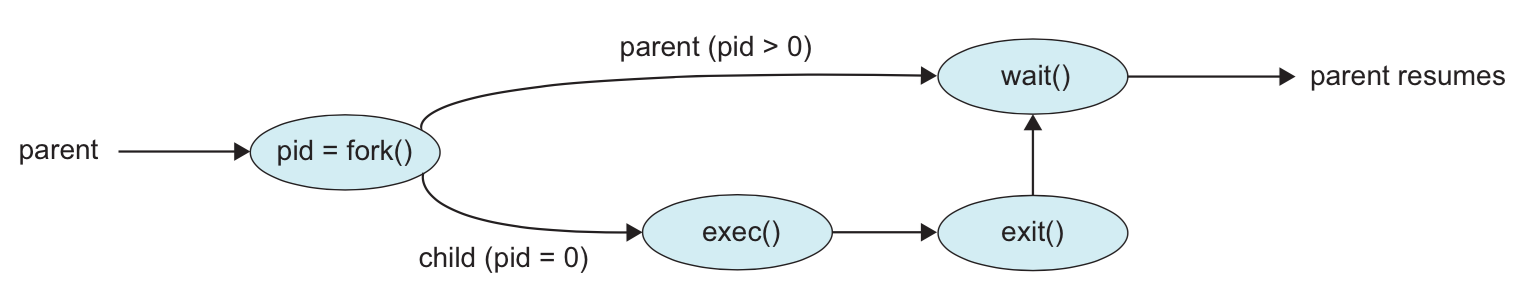
\includegraphics[width=\textwidth]{images/fork-syscall.png}
\end{center}

\end{frame}

\begin{frame}
  \frametitle{Assumptions}


  First, we'll see how to use threads on ``embarrassingly parallel problems''.
  \begin{itemize}
    \item mostly-independent sub-problems (little synchronization); and
    \item strong locality (little communication).
  \end{itemize}
  \vfill
  Later, we'll see:
  \begin{itemize}
    \item which problems can be parallelized (\structure{dependencies})
    \item alternative parallelization patterns\\(right now, just use one thread
          per sub-problem)
  \end{itemize}

\end{frame}
%%%%%%%%%%%%%%%%%%%%%%%%%%%%%%%%%%%%%%%%%%%%%%%%%%%%%%%%%%%%%%%%%%%%%%%%%%%%%%%%

\begin{frame}
  \frametitle{POSIX Threads}


  \begin{itemize}
    \item Available on most systems
    \vfill
    \item Windows has Pthreads Win32, but I wouldn't use it; \\use Linux for
          this course
    \vfill
    \item API available by {\tt \#include <pthread.h>}
    \vfill
    \item Compile with pthread flag \\ ({\tt gcc -pthread prog.c -o prog})
  \end{itemize}

\end{frame}

%%%%%%%%%%%%%%%%%%%%%%%%%%%%%%%%%%%%%%%%%%%%%%%%%%%%%%%%%%%%%%%%%%%%%%%%%%%%%%%%

\begin{frame}[fragile]
  \frametitle{C++ 11 Threads}


  \begin{itemize}
    \item Now part of the C++ standard (library)
    \vfill
    \item API available with {\tt \#include <thread>}
    \vfill
    \item Compile with flags: \\ (\verb!g++ -std=c++11 -pthread prog.c -o prog!)
  \end{itemize}

\end{frame}


%%%%%%%%%%%%%%%%%%%%%%%%%%%%%%%%%%%%%%%%%%%%%%%%%%%%%%%%%%%%%%%%%%%%%%%%%%%%%%%%
\begin{frame}[fragile]
  \frametitle{Pthreads: Creating Threads}


  \begin{lstlisting}
int pthread_create(pthread_t* thread, 
                   const pthread_attr_t* attr,
                   void* (*start_routine)(void*),
                   void* arg);
  \end{lstlisting}
  \vfill
  {\bf thread}: creates a handle to a thread at pointer location

  {\bf attr}: thread attributes (NULL for defaults, more details later)

  {\bf start\_routine}: function to start execution

  {\bf arg}: value to pass to start\_routine
  \vfill
  returns 0 on success, error number otherwise\\(contents of *thread are
  undefined)

\end{frame}
%%%%%%%%%%%%%%%%%%%%%%%%%%%%%%%%%%%%%%%%%%%%%%%%%%%%%%%%%%%%%%%%%%%%%%%%%%%%%%%%

%%%%%%%%%%%%%%%%%%%%%%%%%%%%%%%%%%%%%%%%%%%%%%%%%%%%%%%%%%%%%%%%%%%%%%%%%%%%%%%%
\begin{frame}[fragile]
  \frametitle{Creating Threads---Pthreads Example}


\begin{lstlisting}
#include <pthread.h>
#include <stdio.h>

void* run(void*) {
  printf("In run\n");
}

int main() {
  pthread_t thread;
  pthread_create(&thread, NULL, &run, NULL);
  printf("In main\n");
}
\end{lstlisting}
  \vfill
  Simply creates a thread and terminates\\(usage isn't really right, as we'll
  see.)

\end{frame}
%%%%%%%%%%%%%%%%%%%%%%%%%%%%%%%%%%%%%%%%%%%%%%%%%%%%%%%%%%%%%%%%%%%%%%%%%%%%%%%%

%%%%%%%%%%%%%%%%%%%%%%%%%%%%%%%%%%%%%%%%%%%%%%%%%%%%%%%%%%%%%%%%%%%%%%%%%%%%%%%%
\begin{frame}[fragile]
  \frametitle{Creating Threads---C++11 Example}


\begin{lstlisting}
#include <thread>
#include <iostream>

void run() {
  std::cout << "In run\n";
}

int main() {
  std::thread t1(run);
  std::cout << "In main\n";
  t1.join(); // hang in there...
}
\end{lstlisting}

\end{frame}
%%%%%%%%%%%%%%%%%%%%%%%%%%%%%%%%%%%%%%%%%%%%%%%%%%%%%%%%%%%%%%%%%%%%%%%%%%%%%%%%


%%%%%%%%%%%%%%%%%%%%%%%%%%%%%%%%%%%%%%%%%%%%%%%%%%%%%%%%%%%%%%%%%%%%%%%%%%%%%%%%
\begin{frame}[fragile]
  \frametitle{Waiting for Threads}


  \begin{lstlisting}
int pthread_join(pthread_t thread,
                 void** retval)
  \end{lstlisting}
  \vfill
  {\bf thread}: wait for this thread to terminate (thread must be~joinable).

  {\bf retval}: stores exit status of thread (set by {\tt pthread\_exit}) to
                 the location pointed by *retval. If cancelled, returns
                 {\tt PTHREAD\_CANCELED}. {\tt NULL} is ignored.
  \vfill
  returns 0 on success, error number otherwise.
  \vfill
  {\bf Only call this one time per thread!} Multiple calls on the same thread
  leads to undefined behaviour.

\end{frame}
%%%%%%%%%%%%%%%%%%%%%%%%%%%%%%%%%%%%%%%%%%%%%%%%%%%%%%%%%%%%%%%%%%%%%%%%%%%%%%%%

%%%%%%%%%%%%%%%%%%%%%%%%%%%%%%%%%%%%%%%%%%%%%%%%%%%%%%%%%%%%%%%%%%%%%%%%%%%%%%%%
\begin{frame}[fragile]
  \frametitle{Waiting for Threads---Pthreads example}


\begin{lstlisting}
#include <pthread.h>
#include <stdio.h>

void* run(void*) {
  printf("In run\n");
}

int main() {
  pthread_t thread;
  pthread_create(&thread, NULL, &run, NULL);
  printf("In main\n");
  pthread_join(thread, NULL);
}
\end{lstlisting}
  \vfill
  This now waits for the newly created thread to terminate.

\end{frame}
%%%%%%%%%%%%%%%%%%%%%%%%%%%%%%%%%%%%%%%%%%%%%%%%%%%%%%%%%%%%%%%%%%%%%%%%%%%%%%%%

%%%%%%%%%%%%%%%%%%%%%%%%%%%%%%%%%%%%%%%%%%%%%%%%%%%%%%%%%%%%%%%%%%%%%%%%%%%%%%%%
\begin{frame}[fragile]
  \frametitle{Creating Threads---C++11 Example}


\begin{lstlisting}
#include <thread>
#include <iostream>

void run() {
  std::cout << "In run\n";
}

int main() {
  std::thread t1(run);
  std::cout << "In main\n";
  t1.join(); // aha!
}
\end{lstlisting}

\end{frame}
%%%%%%%%%%%%%%%%%%%%%%%%%%%%%%%%%%%%%%%%%%%%%%%%%%%%%%%%%%%%%%%%%%%%%%%%%%%%%%%%

%%%%%%%%%%%%%%%%%%%%%%%%%%%%%%%%%%%%%%%%%%%%%%%%%%%%%%%%%%%%%%%%%%%%%%%%%%%%%%%%
\begin{frame}[fragile]
  \frametitle{Passing Data to Pthreads threads\ldots Wrongly}


Consider this snippet:
\vfill
\begin{lstlisting}
int i;
for (i = 0; i < 10; ++i)
  pthread_create(&thread[i], NULL, &run, (void*)&i);
\end{lstlisting}
  \vfill
  This is a \alert{terrible} idea. Why?
  \vfill
  \begin{enumerate}
    \item<2-> The value of {\tt i} will probably change before the thread executes
    \item<2-> The memory for {\tt i} may be out of scope, and therefore invalid by
          the time the thread executes
  \end{enumerate}


\end{frame}
%%%%%%%%%%%%%%%%%%%%%%%%%%%%%%%%%%%%%%%%%%%%%%%%%%%%%%%%%%%%%%%%%%%%%%%%%%%%%%%%

%%%%%%%%%%%%%%%%%%%%%%%%%%%%%%%%%%%%%%%%%%%%%%%%%%%%%%%%%%%%%%%%%%%%%%%%%%%%%%%%
\begin{frame}[fragile]
  \frametitle{Passing Data to Pthreads threads}


What about:
\begin{lstlisting}
int i;
for (i = 0; i < 10; ++i)
  pthread_create(&thread[i], NULL, &run, (void*)i);

...

void* run(void* arg) {
  int id = (int)arg;
\end{lstlisting}
  \vfill
  This is suggested in the book, but should carry a warning:

  \vfill
  \begin{itemize}
    \item<2-> Beware size mismatches between arguments: 
      no guarantee that a pointer is the same size as an int, so your data
      may overflow.
    \item<2-> Sizes of data types change between systems. For maximum
      portability, just use pointers you got {\tt from malloc}.
  \end{itemize}


\end{frame}
%%%%%%%%%%%%%%%%%%%%%%%%%%%%%%%%%%%%%%%%%%%%%%%%%%%%%%%%%%%%%%%%%%%%%%%%%%%%%%%%

%%%%%%%%%%%%%%%%%%%%%%%%%%%%%%%%%%%%%%%%%%%%%%%%%%%%%%%%%%%%%%%%%%%%%%%%%%%%%%%%
\begin{frame}[fragile]
  \frametitle{Passing Data to C++11 threads}

It's easier to get data to threads in C++11:
\begin{lstlisting}
#include <thread>
#include <iostream>

void run(int i) {
  std::cout << "In run " << i << "\n";
}

int main() {
  for (int i = 0; i < 10; ++i) {
    std::thread t1(run, i);
    t1.detach(); // see the next slide...
  }
}
\end{lstlisting}

  
\end{frame}
%%%%%%%%%%%%%%%%%%%%%%%%%%%%%%%%%%%%%%%%%%%%%%%%%%%%%%%%%%%%%%%%%%%%%%%%%%%%%%%%

%%%%%%%%%%%%%%%%%%%%%%%%%%%%%%%%%%%%%%%%%%%%%%%%%%%%%%%%%%%%%%%%%%%%%%%%%%%%%%%%
\begin{frame}[fragile]
  \frametitle{Getting Data from C++11 threads}

    \ldots but it's harder to get data back.\\
    Use {\tt async} and {\tt future} abstractions:
    \begin{lstlisting}
#include <thread>
#include <iostream>
#include <future>

int run() {
  return 42;
}

int main() {
  std::future<int> t1_retval =
                  std::async(std::launch::async, run);
  std::cout << t1_retval.get();
}
\end{lstlisting}

  
\end{frame}
%%%%%%%%%%%%%%%%%%%%%%%%%%%%%%%%%%%%%%%%%%%%%%%%%%%%%%%%%%%%%%%%%%%%%%%%%%%%%%%%

%%%%%%%%%%%%%%%%%%%%%%%%%%%%%%%%%%%%%%%%%%%%%%%%%%%%%%%%%%%%%%%%%%%%%%%%%%%%%%%%
\begin{frame}[fragile]
  \frametitle{Detached Threads}


  {\it Joinable} threads (the default) wait for someone to call
  {\tt pthread\_join} before they release their resources.
  \vfill
  {\it Detached} threads release their resources when they terminate, without
  being joined.
  \vfill
  \begin{lstlisting}
int pthread_detach(pthread_t thread);
  \end{lstlisting}
  \vfill
  {\bf thread}: marks the thread as detached
  \vfill
  returns 0 on success, error number otherwise.
  \vfill
  Calling {\tt pthread\_detach} on an already detached thread results in undefined
  behaviour.


\end{frame}
%%%%%%%%%%%%%%%%%%%%%%%%%%%%%%%%%%%%%%%%%%%%%%%%%%%%%%%%%%%%%%%%%%%%%%%%%%%%%%%%

%%%%%%%%%%%%%%%%%%%%%%%%%%%%%%%%%%%%%%%%%%%%%%%%%%%%%%%%%%%%%%%%%%%%%%%%%%%%%%%%
\begin{frame}[fragile]
  \frametitle{Thread Termination}


  \begin{lstlisting}
void pthread_exit(void *retval);
  \end{lstlisting}
  \vfill
  {\bf retval}: return value passed to function that calls {\tt pthread\_join}
  \vfill
  start\_routine returning is equivalent to calling {\tt pthread\_exit} with
  that return value;
  \vfill
  {\tt pthread\_exit} is called implicitly when the {\tt start\_routine} of a
  thread returns.
  \vfill
  There is no C++11 equivalent.


\end{frame}
%%%%%%%%%%%%%%%%%%%%%%%%%%%%%%%%%%%%%%%%%%%%%%%%%%%%%%%%%%%%%%%%%%%%%%%%%%%%%%%%

%%%%%%%%%%%%%%%%%%%%%%%%%%%%%%%%%%%%%%%%%%%%%%%%%%%%%%%%%%%%%%%%%%%%%%%%%%%%%%%%
\begin{frame}
  \frametitle{Attributes}


  By default, threads are {\it joinable} on Linux, but a more portable way to
  know what you're getting is to set thread attributes. You can change:
  \begin{itemize}
    \item Detached or joinable state
    \item Scheduling inheritance
    \item Scheduling policy
    \item Scheduling parameters
    \item Scheduling contention scope
    \item Stack size
    \item Stack address
    \item Stack guard (overflow) size
  \end{itemize}


\end{frame}
%%%%%%%%%%%%%%%%%%%%%%%%%%%%%%%%%%%%%%%%%%%%%%%%%%%%%%%%%%%%%%%%%%%%%%%%%%%%%%%%

%%%%%%%%%%%%%%%%%%%%%%%%%%%%%%%%%%%%%%%%%%%%%%%%%%%%%%%%%%%%%%%%%%%%%%%%%%%%%%%%
\begin{frame}[fragile]
  \frametitle{Attributes---Example}


  \begin{lstlisting}
size_t stacksize;
pthread_attr_t attributes;
pthread_attr_init(&attributes);
pthread_attr_getstacksize(&attributes, &stacksize);
printf("Stack size = %i\n", stacksize);
pthread_attr_destroy(&attributes);
  \end{lstlisting}
Running this on a laptop produces:
  \begin{lstlisting}
jon@riker examples master % ./stack_size 
Stack size = 8388608
  \end{lstlisting}
  Setting a thread state to joinable:
  \begin{lstlisting}
pthread_attr_setdetachstate(&attributes,
                            PTHREAD_CREATE_JOINABLE);
  \end{lstlisting}


\end{frame}
%%%%%%%%%%%%%%%%%%%%%%%%%%%%%%%%%%%%%%%%%%%%%%%%%%%%%%%%%%%%%%%%%%%%%%%%%%%%%%%%

%%%%%%%%%%%%%%%%%%%%%%%%%%%%%%%%%%%%%%%%%%%%%%%%%%%%%%%%%%%%%%%%%%%%%%%%%%%%%%%%
\begin{frame}[fragile]
  \frametitle{Detached Threads: Warning!}


\begin{lstlisting}
#include <pthread.h>
#include <stdio.h>

void* run(void*) {
  printf("In run\n");
}

int main() {
  pthread_t thread;
  pthread_create(&thread, NULL, &run, NULL);
  pthread_detach(thread);
  printf("In main\n");
}
\end{lstlisting}

  When I run it, it just prints ``In main'', why?


\end{frame}
%%%%%%%%%%%%%%%%%%%%%%%%%%%%%%%%%%%%%%%%%%%%%%%%%%%%%%%%%%%%%%%%%%%%%%%%%%%%%%%%

%%%%%%%%%%%%%%%%%%%%%%%%%%%%%%%%%%%%%%%%%%%%%%%%%%%%%%%%%%%%%%%%%%%%%%%%%%%%%%%%
\begin{frame}[fragile]
  \frametitle{Detached Threads: Solution to Problem}

  \begin{lstlisting}
#include <pthread.h>
#include <stdio.h>

void* run(void*) {
  printf("In run\n");
}

int main() {
  pthread_t thread;
  pthread_create(&thread, NULL, &run, NULL);
  pthread_detach(thread);
  printf("In main\n");
  pthread_exit(NULL); // This waits for all detached
                      // threads to terminate
}
  \end{lstlisting}

  Make the final call {\tt pthread\_exit} if you have any detached threads. (There is no C++11 equivalent.)

\end{frame}
%%%%%%%%%%%%%%%%%%%%%%%%%%%%%%%%%%%%%%%%%%%%%%%%%%%%%%%%%%%%%%%%%%%%%%%%%%%%%%%%

%%%%%%%%%%%%%%%%%%%%%%%%%%%%%%%%%%%%%%%%%%%%%%%%%%%%%%%%%%%%%%%%%%%%%%%%%%%%%%%%
\begin{frame}
  \frametitle{Threading Challenges}

  \begin{itemize}
    \item Be aware of scheduling (you can also set affinity with pthreads on
      Linux).
    \vfill
    \item Make sure the libraries you use are {\bf thread-safe}:
      \begin{itemize}
        \item Means that the library protects its shared data.
      \end{itemize}
    \vfill
    \item glibc reentrant functions are also safe: a program can have more than one
      thread calling these functions concurrently.
    \vfill
    \item {\bf Example:} {\tt rand\_r} versus
      {\tt rand}.
  \end{itemize}

\end{frame}
%%%%%%%%%%%%%%%%%%%%%%%%%%%%%%%%%%%%%%%%%%%%%%%%%%%%%%%%%%%%%%%%%%%%%%%%%%%%%%%%




\end{document}

